\chapter{Implementation}
\label{sec:implementation}

In this section we present details about our implementation, including a
prototype framework and three non-trivial wide-area streaming applications.
\sysname{} is implemented in Rust and open-source on Github.\footnote{Url elided
  for anonymity.}

\section{Framework}
\label{sec:framework}

While our proposed APIs are general and not language specific, we chose a safe
language, Rust, for the core framework for the following reasons. First, Rust's
memory safety guarantee can ensure applications running continously for an
extended period of time. Besides, the zero-cost abstraction removes the
possibilities of tail latencies caused by uncoordinated garbage
collection~\cite{maas2016taurus}. In addition, we rely on Rust's type system to
enforce the type match on \texttt{maybe} operations.

\begin{sloppypar}
All operators implement the \texttt{Stream} trait which has an associate type
\texttt{Item} and a core function \texttt{next} that returns
\texttt{Datum}. Each datum is either an item with the \texttt{Stream::Item} or
an \texttt{Error} that the operator use to communicate with the runtime
scheduler. The concrete form of \texttt{maybe} API is almost an direct
translation of the API specification. While our API specification
in~\autoref{tab:operators} uses a vector for knobs, our Rust implementation is
more general: any type (including vector) that implements \texttt{IntoKnob}
trait can be used as the knob.
\end{sloppypar}

\begin{lstlisting}
pub trait Stream {
    type Item;
    fn next(&mut self) -> Datum<Self::Item, Error>;

    fn maybe<K, F>(self, opts: K, f: F) -> Maybe<Self, F>
        where Self: Sized,
                K: IntoKnob,
                F: FnMut(K::Item, Self::Item) -> Self::Item {

         // omitted
    }
}

pub trait IntoKnob {
    fn into_knob(self) -> Knob;
}
\end{lstlisting}

Developers can directly use the above API with user-defined functions. The
snippet below shows how a quantization degradation can be implemented with our
API. First, a vector of values is converted into a stream object. Then a
\texttt{maybe} operator with a knob value (2 or 3) and a function that performs
an interger division (quantization). Function \texttt{collect} will run this
stream and hold the output in a vector. Depending on the degradation level, the
output stream could either be [1, 2, 3, 4], [0, 1, 1, 2], or [0, 0, 1, 1].

\begin{lstlisting}
let quantized_stream = vec![1, 2, 3, 4]
    .into_stream()
    .maybe(vec![2, 3], |knob, p| p / knob);
    .collect();
\end{lstlisting}

We've also extended the basic API for common operations. As we are building
video processing applications, we implemented a specialized
\texttt{maybe\_downsample} operator can that wraps \texttt{downsample} function
internally.

\begin{lstlisting}
fn downsample(res: (usize, usize), image: Mat) -> Mat {

    //  omitted

}
\end{lstlisting}

Applications built with \sysname{} runs as a single process. The entire
processing pipeline is often specified in a single main file. The execution mode
(profiling, runtime as client or runtime as server) is configured with command
line arguments or environment variables. Our deployment manager is currently a
shell script using Docker container.

\section{Building \sysname{} Applications}
\label{sec:build-appl}

Using \sysname{}, we've built three applications: pedestrian detection
surveillance, an augmented reality and a distributed Top-k (\autoref{fig:apps}).
\autoref{tab:apps} summarizes the application specific part: knobs, utility
function and dataset

\begin{table*}
  \small
  \centering
  \begin{tabular}{|c|c|c|c|}
    \hline
    Application & Knobs & Utility & Dataset \\
    \hline
    Pedestrian Detection & resolution, framerate, quantizer
                        & F1 score & MOT16-04 (training), MOT16-03 (testing) \\
    \hline
    Augmented Reality & resolution, framerate, quantizer
                        & F1 score & Video clips of office (training), home (testing) \\
    \hline
    Top-K & head (N), local threshold (T) & Kendall's W & sec.gov access log
                                                          (4 days training, 12 days testing)  \\
    \hline
  \end{tabular}
  \caption{\sysname{} Applications}
  \label{tab:apps}
\end{table*}

\begin{figure*}
  \centering
  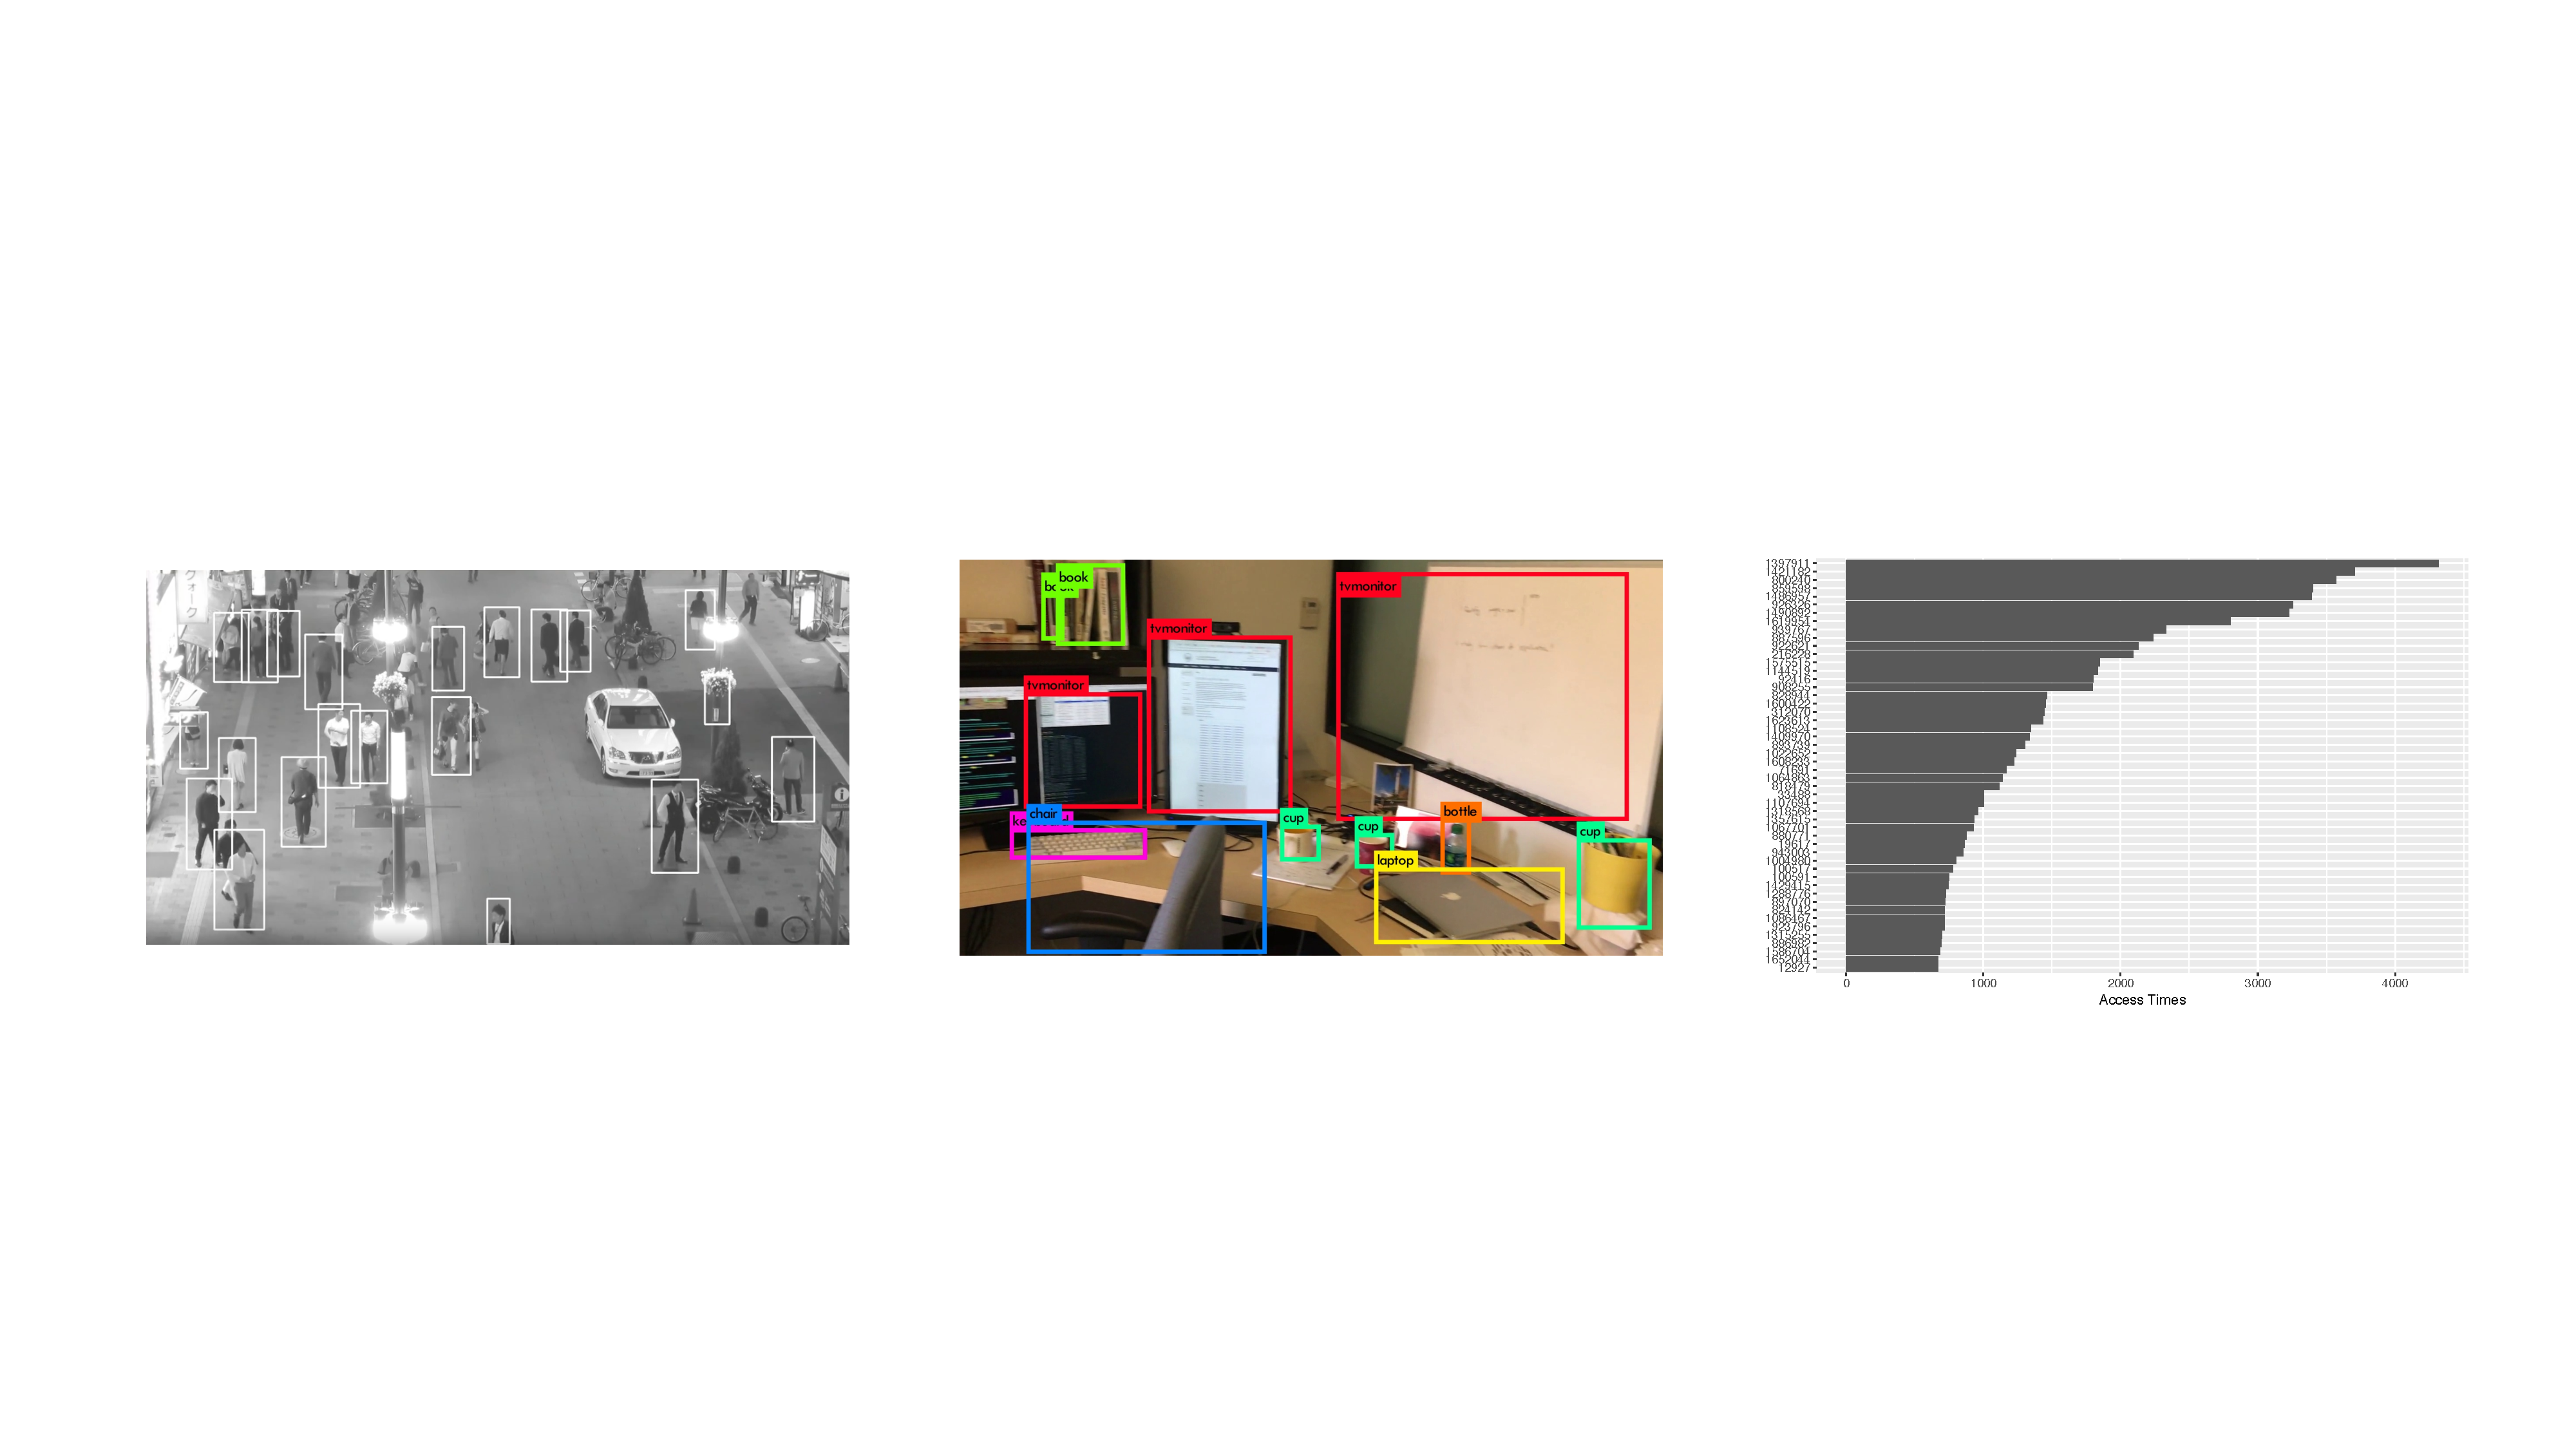
\includegraphics[width=.95\textwidth]{figures/apps.pdf}
  \caption{\sysname{} applications}
  \label{fig:apps}
\end{figure*}

\para{Pedestrian Detection:} This application analyzes video streams from
installed CCTV cameras and detect pedestrians inside. The detection result is a
list of bounding boxes representing pedestrian's relative location within the
view. Variant of this application can be used for safety monitoring, anomaly
detection or waiting line counting.

We implement most image-related operations with OpenCV
3.1~\cite{opencvlibrary}. Pedestrians are detected using histogram of oriented
gradients (HOG)~\cite{dalal2005histograms} with the default linear SVM
classifier. To ensure real-time processing of frames, GPU-accelerated
implementation is used in favor of the CPU-based implementation.

For video encoding, H.264 scheme is chosen for its prevalence in existing
systems. Our implemenation is based on GStreamer~\cite{gstreamer}, using
\texttt{x264enc} plugin. To integrate with \sysname{}, we first create a
pipeline that exposes \texttt{appsrc} (to feed raw image data) and
\texttt{appsink} (to get encoded bytes). The GStreamer main loop is managed in a
separate thread and \sysname{} communicates with it via Rust's channel. The
\texttt{x264enc} is configured with \texttt{zerolatency} present and runs using
four threads. It uses constant quality encoding and the quantizer is exported as
a parameter that can be tuned.

This application has three degradation operations: reducing image resolution,
dropping frame rate or lower video encoding quality.

The detection returns a list of bounding boxes; it's compared against a
reference result (either the groundtruth or the one without degradation). A
successful detection is defined when the intersection over union (IOU) is
greater than 50\%~\cite{everingham2010pascal}. For the utility function, we use
F1 score (\%), the harmonic mean of precision and
recall~\cite{Rijsbergen:1979:IR:539927}.

\para{Augmented Reality:} We target at mobile augmented reality applications
which offload the heavy computation to resources elsewhere. Although local
computation is gaining attraction~\cite{satyanarayanan2009case, zhang2015cloud},
wireless communication link is also susceptible to capacity variation.

We use a similar setup as the pedestrian detection application except the actual
function that analyzes the stream. To recognize objects, we use a a pre-trained
neural network~\cite{darknet13} that's trained with
Imagenet~\cite{krizhevsky2012imagenet}. Similar to our first application,
GPU-accelerated implementation is use in favor for real-time processing.

The utility function here is more strict than the pedestrian detection:
true-positive depends not only on IOU criteria, but also on the type of objects
(a correct identification).

\para{Distributed Top-K:} Many distributed system monitoring applications
require to answer the ``top-k'' question~\cite{babcock2003distributed}, such as
the top-k most popular URLs or the top-k most access files. Naive methods of
transmitting all the raw log entries to the aggregation point is not feasible as
popular servers typically have millions of requests per second. Local worker
node can first perform a window-based transformation that generates data
summary, such as key-value pairs of \texttt{<item, count>}. However, even after
this operation, the data size could still be too large given most real-world
access patterns follow a long-tailed distribution. There is a
large-but-irrelevant tail that is unnecessary to send.

We consider two degradation operations that individual worker nodes can perform:
(1) a local Top-\texttt{N} operation that shortens the list first; (2) a local
threshold \texttt{T} that further filters small entries. Obviously, these two
operations are not orthognal to each other. Their impact on data size reduction
and quality degradation depends on the distribution of the actual data.

\begin{figure}
  \centering
  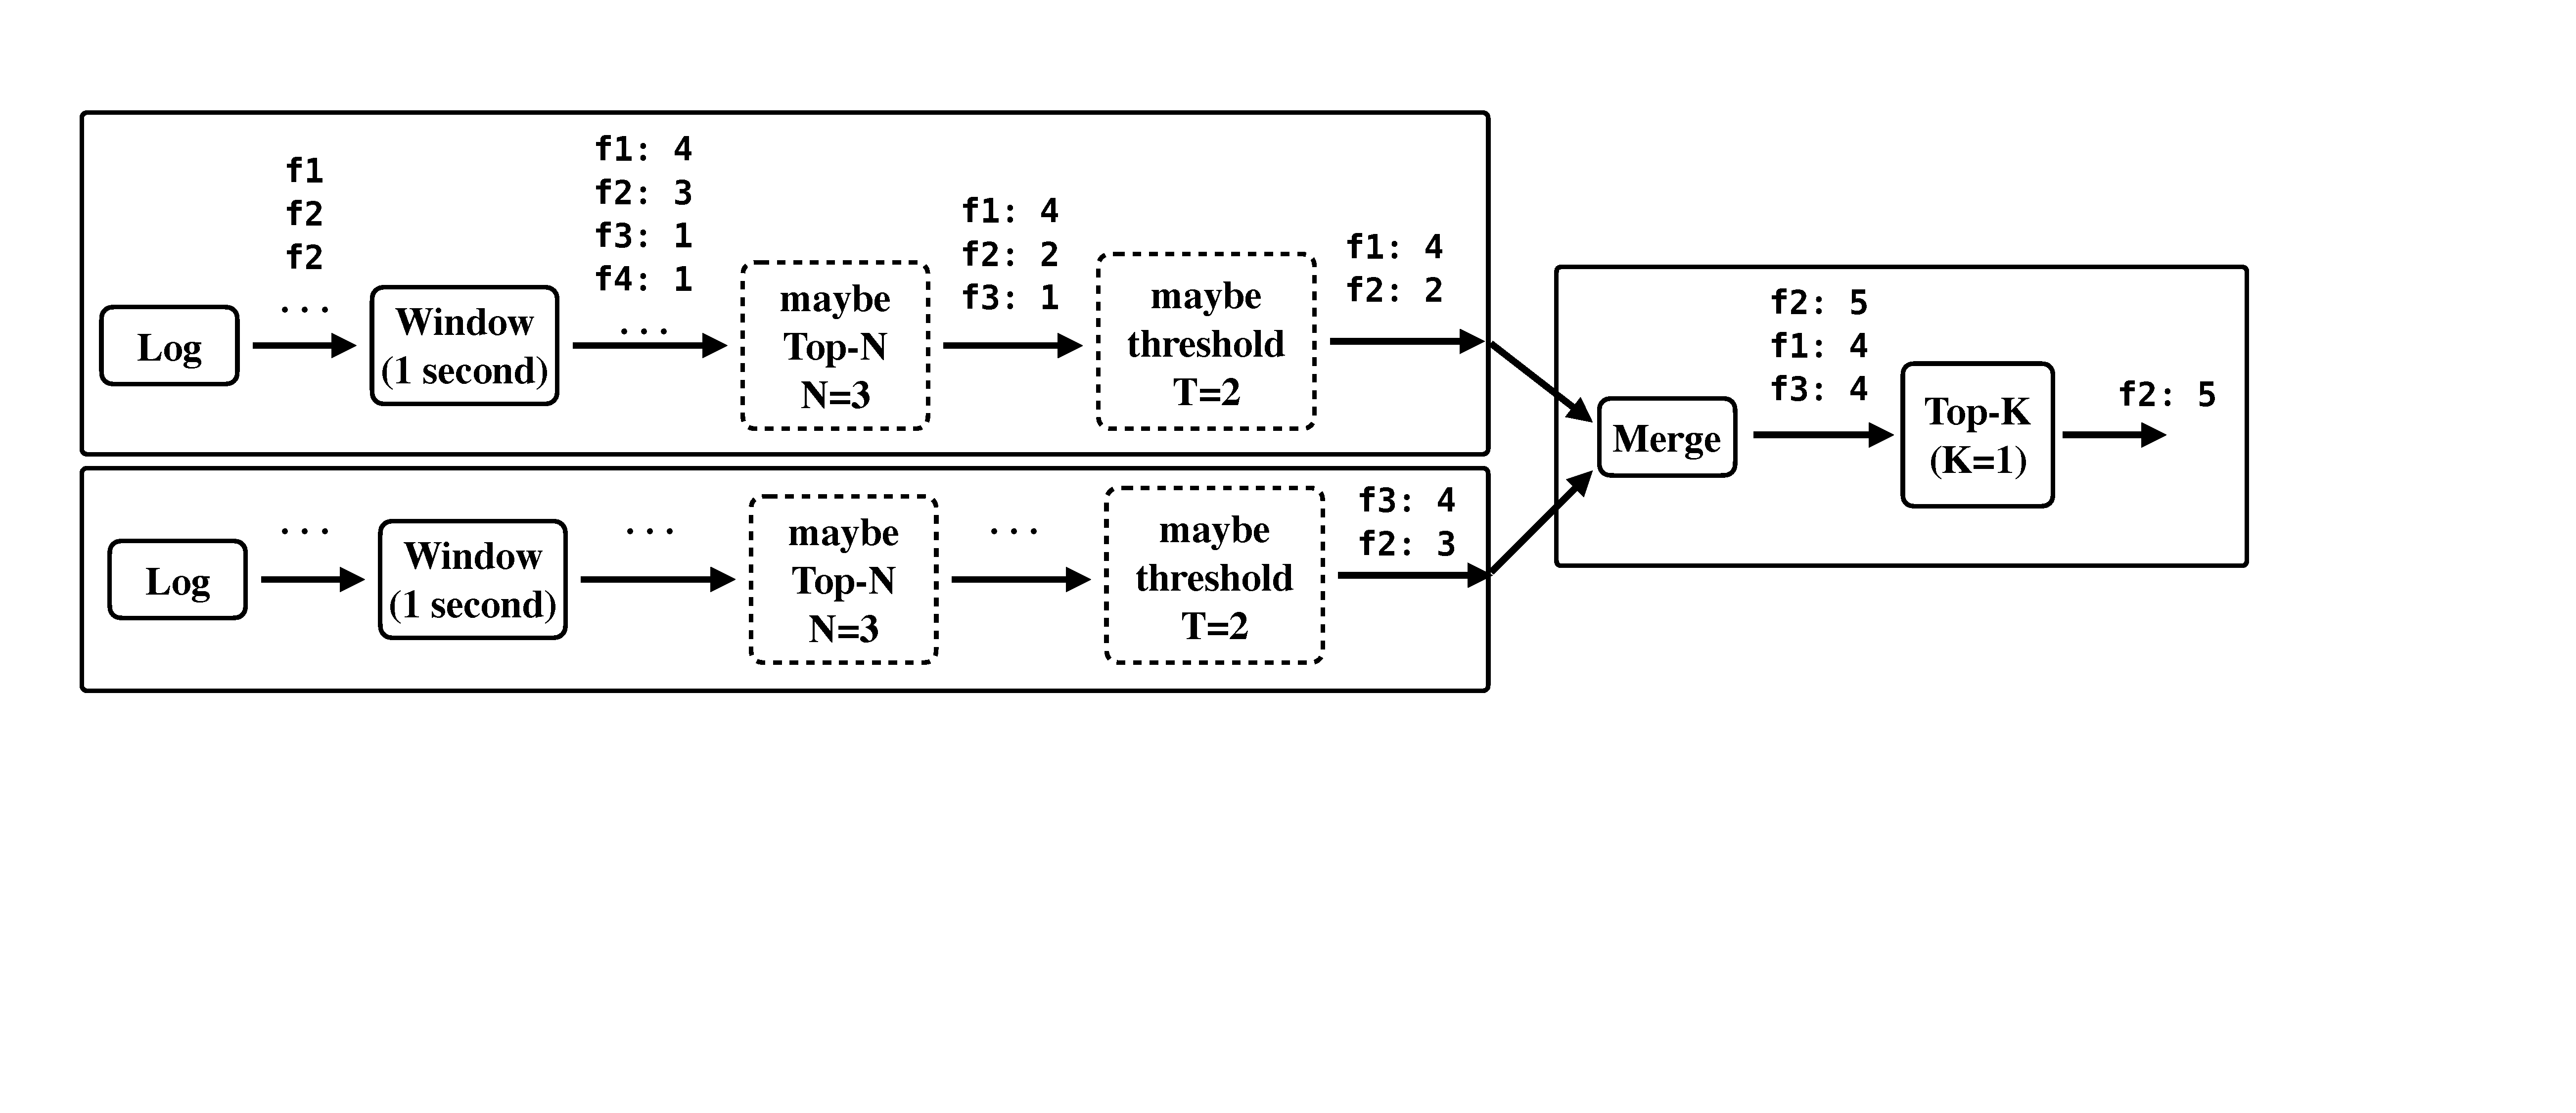
\includegraphics[width=\linewidth]{figures/topk.pdf}
  \caption{A distributed Top-K application has two tunable parameters: a local
    Top-N (N) and a local threshold (T).}
  \label{fig:topk}
\end{figure}


we use Kendall's W as the utility function here. It is a distance measure of the
concordance between two ranked list. The function outputs a statistic measure
ranging from 0 to 1, representing no agreement to complete aggrement,
respectively~\cite{abdi2007kendall}.


\section{Evaluation}
\label{sec:evaluation}

We first show the generated profile for the three applications. Then for each
application, We show how they adapt the behavior at runtime. Under a controlled
experiment, even with only transient network capacity drop, our system is able
to maintain an end-to-end delay for 10 seconds in the wide-area and accuracy
level above 80\%. Application-agnostic protocols creates significant backlogged
data (TCP for about 100 seconds) or unusable accuracy (UDP).

\subsection{Degradation Performance}
\label{sec:degr-perf}

\begin{figure}
  \centering
  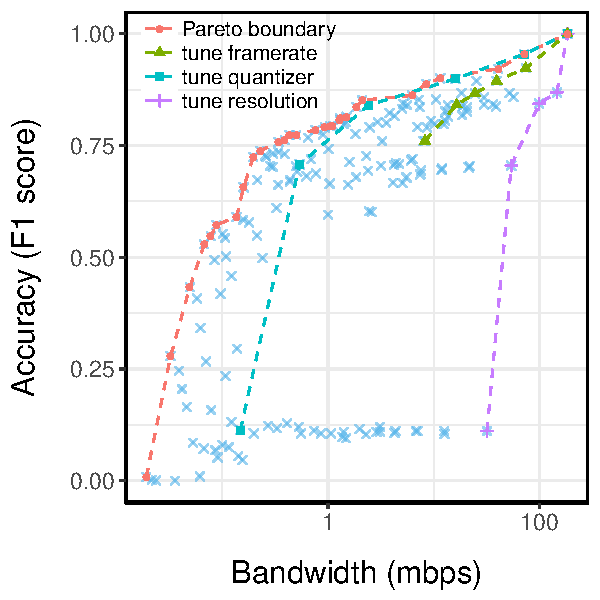
\includegraphics[width=0.6\textwidth]{figures/ped-profile.pdf}
  \caption{Pedestrian Detection}
  \label{fig:pd-profile}
\end{figure}

\begin{figure}
  \centering
  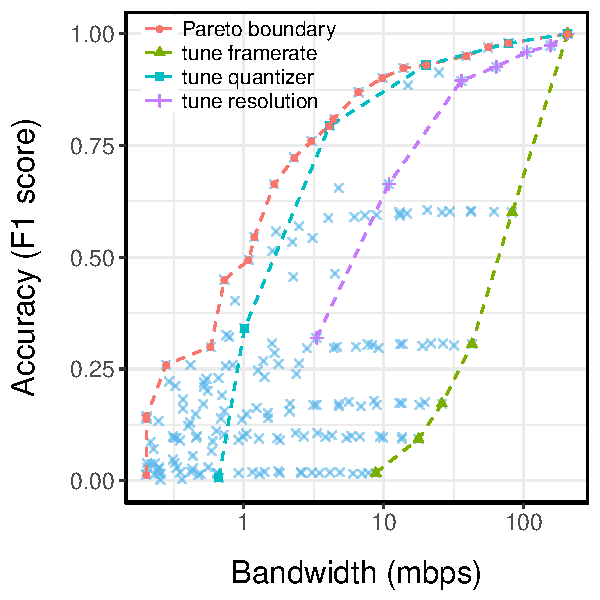
\includegraphics[width=0.6\textwidth]{figures/darknet-profile.pdf}
  \caption{Augmented Reality}
  \label{fig:ar-profile}
\end{figure}

\begin{figure}
  \centering
  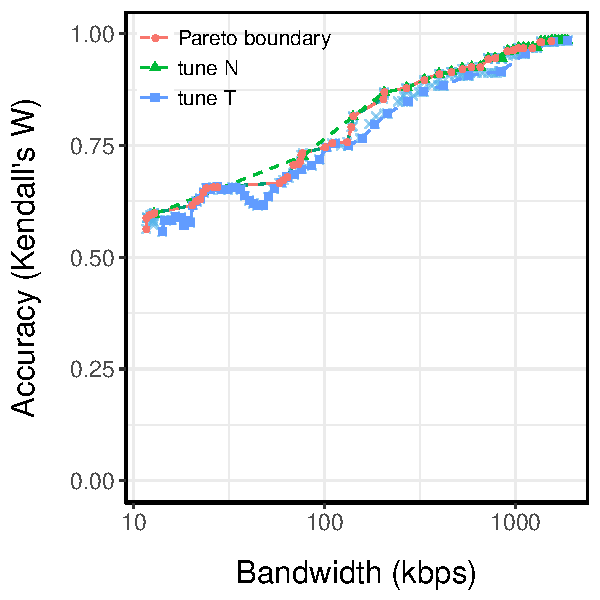
\includegraphics[width=0.6\textwidth]{figures/log-profile.pdf}
  \caption{Top-k}
  \label{fig:tk-profile}
\end{figure}

We describe the dataset we used for offline profiling and interpret the
profiling results (\autoref{fig:all-profiles}) in turn.

\para{Pedestrian Detection:} We use MOT16 dataset~\cite{milan2016mot16} to
evaluate this application. Specifically we used MOT16-04 as the training
dataset. The video feeds capture a busy pedestrian street at night with an
elevated viewpoint. The original resolution is 1920x1080, with frame rate
30. The training data has 1050 frames in total, amounting 35-second monitoring.
On averge there are 45.3 people per frame.

There are three knobs in this application: resolution, frame rate and encoding
quality. To maintain the same 16:9 aspect ratio with the original 1920x1080
resolution, the first degradation only chooses common 16:9 resolutions:
1600x900, 1280x720, 960x540, 640x320. For the framerate, integer values are
chosen in favor of fraction values. The original frame rate is 30, and our
degradation explores 10, 5, 3, 2, 1. H.264 encoding quantizer has a range from 0
(lossless) to 51 (worst possible), and 18 is the visually
lossless~\cite{bellard2012ffmpeg}. In our experiment, we use 10, 20, 30, 40, 50
as degradation parameters.

The generated profile is shown in~\autoref{fig:pd-profile} with x-axis the
required bandwidth and the y-axis the accuracy (F1 score). Note the log scale on
the horizontal axis as raw uncompressed 8-bit RGB video streams are
prohibitively large: $1920 \times 1080 \times 30 \times 3 \times 8 = 1.5 $ Gbps.

Each point in the scatter plot represents one configuration that our offline
profiling has evaluated. Notice the vast spread in bandwidth requirement among
configurations with similar accuracy as well as the wide spread in accuracy
among configurations that consumes similar bandwidth.

We first show three lines in the case of only tuning one knob. Notice the
distinct behavior of the three lines. In this particular application, reducing
the resolution has the most penalty because the HOG detector has a minimal 128
pixels by 64 pixels window. The camera is deployed in a far-field context;
scaling down the image will quickly has an effect on the detection. Tuning frame
rate doesn't affect the accuracy too much. In fact, even with 1 FPS, the
accuracy is still relatively high. However, reducing frame rate doesn't bring
much bandwidth saving (as we have mentioned in \autoref{fig:h264}).  The most
effective way that reduces the bandwidth while preserving the accuracy is to
adjust the quantizer because it affects almost every pixel and creates smaller
P-frames.

The Pareto boundary, or \textit{profile}, is the most important curve. In the
begining it's close to the curve when only quantizer is tuned, quantizer has a
certain limit. A crisp image is prefered as many image processing algorithms are
looking for the edges while for human consumption, a smoother image is fine.

As the uncompressed video is not practical, we imposes a bandwidth cap before
the profile is used in runtime (only use optimal configurations that creates
video with less than 20mbps data rate).

\para{Augmented Reality:} We collected training set for this application
ourselves. It's a 23-second video clip with 1920x1080 resolution and 30 FPS
taken on a mobile phone. During the capture, we change the camera view in a slow
pace to emulate how a real user would look around. Because target objects are
relatively close while the camera is moving, we hypothesis for this training
set, the profile will be different from the previous application that reducing
frame rate will have a detrimental effect.

The generate profile is shown in \autoref{fig:ar-profile}. First, we see our
intuition backed up by measurements. Besides, the Pareto boundary also first
follows the video encoding knob, but optimal settings are achieved only when
multiple degradations are in effect.

\para{Top-K:} To evalute the top-k application, we generate synthetic dataset
based on real-world access logs (EDGAR log file dataset, the access log of
\url{https://sec.gov}). The original log contains CSV-format data extract from
Apache web server that records and stores user access
statistics~\cite{edgarlog}. The original log has only 500k access per hour; it's
rather small in comparison to today's CDN log. We condensed an hour-long data
into one second. After performing the local aggregation, the data size is
reduced from 500k entries per second to 50k key-value pairs (10x reduction).
Next we explore the space of degradation with respect to parameter N and T.  The
parameter N is from 100 to 15000; T from 0 to 500.

\autoref{fig:tk-profile} shows the generated profile. As we can see, most
configurations are very close to the pareto boundary. In the case when data skew
is more severe, we might see that T is more severe. Regardless, with our
automatic profiling tool, developers don't have to thoroughly understand the
complex relationship between bandwidth, accuracy and configuration.

\subsection{Runtime Performance}
\label{sec:runtime-performance}

\begin{figure*}
  \centering
  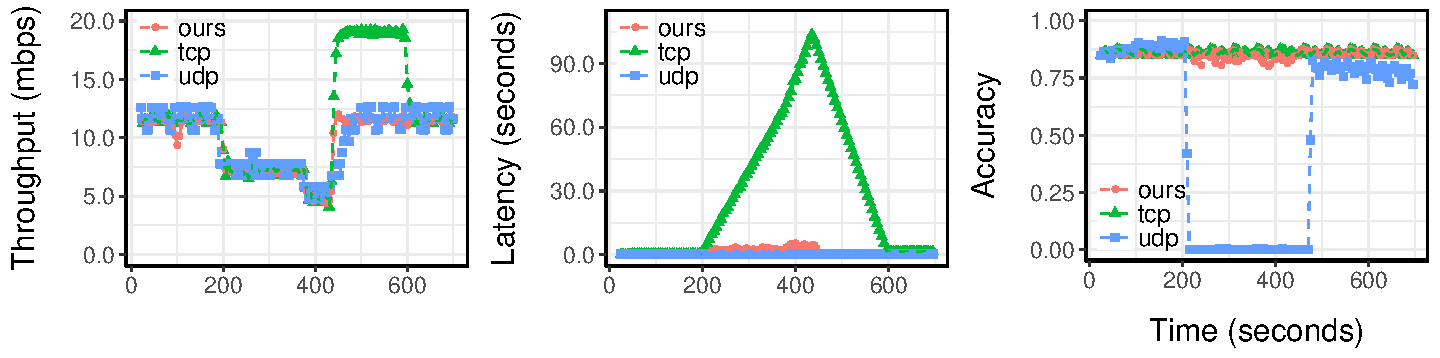
\includegraphics[width=0.95\textwidth]{figures/ped-runtime-horizontal.pdf}
  \caption{Runtime Adaptation of Pedestrian Detection}
  \label{fig:ped-runtime}
\end{figure*}

\begin{figure*}
  \centering
  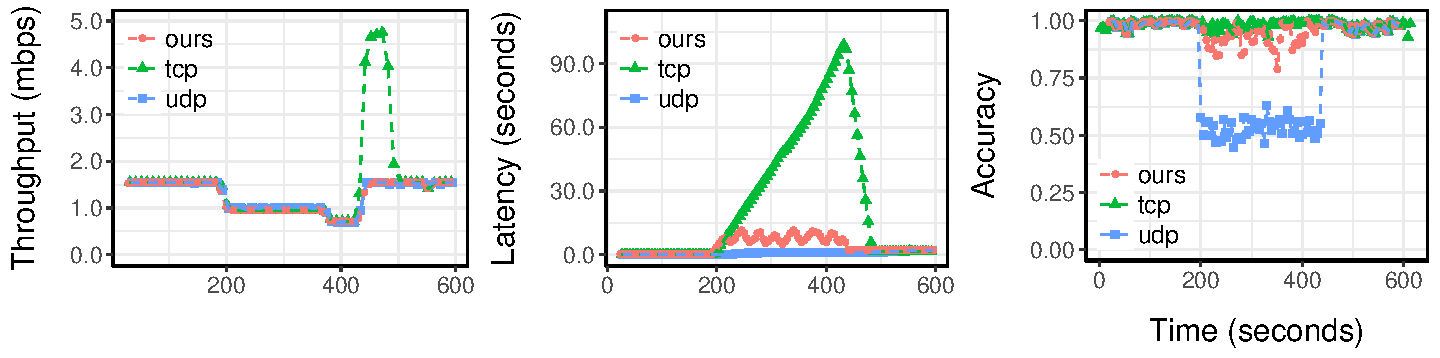
\includegraphics[width=0.95\textwidth]{figures/cdn-runtime-horizontal.pdf}
  \caption{Runtime Adaptation of Top-K}
  \label{fig:ped-runtime}
\end{figure*}

To evaluate the runtime behavior, we conduct controlled experiments using four
geo-distributed worker nodes from Amazon EC2 (t2.large instances) and an
aggregation server from our institute. For each experiment, worker nodes
transmit test data for about 10 mins. During each session, we use Linux
\texttt{tc} utility to adjust outgoing bandwidth to experiment with network
resource variation.

We compare our system with baseline systems that directly uses TCP and UDP. In
all three applications, the raw data streams are orders of magnitude
larger. While our system can adapt the rate, it could be unfair to baseline
solutions. We adjust the default degradation operation so that TCP and UDP would
work just fine when in normal cases; in this way, we make fair comparison. In
the case of UDP, shaping at the source doesn't emulate the packet loss behavior
with out-of-order delivery. We use \texttt{netem} to control packet loss rate to
match the desired shaping bandwidth.

In all three experiments, we see long delays in TCP. It increases linearly when
the traffic shaping started. When the bandwidth shaping stops, TCP quickly fills
the connection to recover. Depending on the queued size, the recovery could take
a few minutes or tens of seconds.

For UDP, the latency has been consistently small (mostly below 1 second) because
there is no queue building up. But when traffic shaping starts, the accuracy
drop is catastrophic.

Applications built with \sysname{} performs with a middle-ground behavior
between two extremes. We notice that our delay is still on the order of ten
seconds. The reason for the slow adaptation is three-folds: (1) our current
implementation only requests for bandwidth information when congestion is
detected, the delay of getting bandwidth estimation can be large in the case of
network capacity drop; (2) we perform the bandwidth in a conservative way with
smoothing to avoid sudden spikes. While more improvements are possible, the
current settings are satisfactory.

%%% Local Variables:
%%% mode: latex
%%% TeX-master: "thesis"
%%% End:
